\subsection{Qualitative Auswertung}

\todo[noline]{Zahlenformat überprüfen}

Im Rahmen der Testsitzungen wurden 20 verschiedene Usability-Probleme identifiziert. Diese wurden entweder im Zuge von \ac{CTA} von den Teilnehmer:innen bemängelt, oder durch Verwirrung, Zögern und fehlerhafte Nutzung festgestellt.

\begin{figure}[!ht]
  \colorlet{presentation}{plot1}
  \colorlet{interaction}{plot2}
  \colorlet{content}{plot3}
  \colorlet{technical}{plot4}
  \centering
  \begin{tikzpicture}
    \begin{axis}[
        xbar=0pt,
        xmajorgrids=true,
        xtick={0,...,10},
        xmin=0,
        xmax=6,
        xlabel={Absolute Häufigkeit},
        /pgf/bar shift=0pt,
        legend style={legend cell align=left},
        legend pos=south east,
        axis y line*=none,
        axis x line*=bottom,
        tick label style={font=\footnotesize},
        legend style={font=\footnotesize},
        label style={font=\footnotesize},
        width=.6\textwidth,
        bar width=3.5mm,
        ymin=1,
        ytick={1,...,20},
        ytick style={draw=none},
        yticklabels={
            {\hyperref[p:functionlist]{Übersichtlichkeit Funktionsliste (T)}},
            {\hyperref[p:präfix]{Präfix von Objektklassen (S)}},
            {\hyperref[p:functions]{Details zu Funktionen (R)}},
            {\hyperref[p:queryables]{Benennung Abfragbare Felder (Q)}},
            {\hyperref[p:meta]{Metadaten von Szenario-Feldern (P)}},
            {\hyperref[p:scroll]{Probleme mit Scrollen (O)}},
            {\hyperref[p:quelle]{Zugriff auf die Quelldaten (N)}},
            {\hyperref[p:filter]{Automatische Typfilterung (M)}},
            {\hyperref[p:statisch]{Angabe von statischen Werten (L)}},
            {\hyperref[p:overload]{Auswahl von Überladungen (K)}},
            {\hyperref[p:mitte]{Benennung mittlerer Bereich (J)}},
            {\hyperref[p:speichern]{Benennung des Speichern-Buttons (I)}},
            {\hyperref[p:parameterübernahme]{Parameterübernahme bei Überladungen (H)}},
            {\hyperref[p:drag]{Drag \& Drop (G)}},
            {\hyperref[p:ersetzen]{Ersetzen von Einträgen (F)}},
            {\hyperref[p:parameter]{Details zu Parametern (E)}},
            {\hyperref[p:attribute]{Anzeige von Attributen in Ziel (D)}},
            {\hyperref[p:datentyp]{Datentyp von Szenario-Feldern (C)}},
            {\hyperref[p:icons]{Icons für Datentypen (B)}},
            {\hyperref[p:bedienreihenfolge]{Bedienreihenfolge von Funktionen (A)}},
          },
        area legend,
        y=6mm,
        enlarge y limits={abs=0.625},
        every axis plot/.append style={fill}
      ]
      \addplot[interaction]  coordinates {(0,0)};  \addlegendentry{Interaktion (8)}
      \addplot[presentation] coordinates {(0,0)};  \addlegendentry{Darstellung (7)}
      \addplot[content]      coordinates {(0,0)};  \addlegendentry{Inhalt (4)}
      \addplot[technical]    coordinates {(0,0)};  \addlegendentry{Technisch (1)}

      \addplot[presentation] coordinates {(1,1)};  % Übersichtlichkeit Funktionsliste
      \addplot[content]      coordinates {(2,2)};  % Präfix von Objektklassen
      \addplot[content]      coordinates {(2,3)};  % Details zu Funktionen
      \addplot[presentation] coordinates {(2,4)};  % Benennung Abfragbare Felder
      \addplot[presentation] coordinates {(2,5)};  % Metadaten von Szenario-Feldern
      \addplot[technical]    coordinates {(3,6)};  % Probleme mit Scrollen
      \addplot[content]      coordinates {(3,7)};  % Zugriff auf die Quelldaten
      \addplot[interaction]  coordinates {(3,8)};  % automatische Typfilterung
      \addplot[interaction]  coordinates {(3,9)}; % Angabe von statischen Werten
      \addplot[interaction]  coordinates {(3,10)};  % Auswahl von Überladungen
      \addplot[presentation] coordinates {(4,11)}; % Benennung mittlerer Bereich
      \addplot[presentation] coordinates {(4,12)}; % Benennung des Speichern-Buttons
      \addplot[interaction]  coordinates {(4,13)}; % Parameterübernahme bei Überladungen
      \addplot[interaction]  coordinates {(4,14)}; % Drag \& Drop
      \addplot[interaction]  coordinates {(4,15)}; % Ersetzen von Einträgen
      \addplot[content]      coordinates {(5,16)}; % Details zu Parametern
      \addplot[presentation] coordinates {(5,17)}; % Anzeige von Attributen in Ziel
      \addplot[interaction]  coordinates {(5,18)}; % Datentyp von Szenario-Feldern
      \addplot[presentation] coordinates {(6,19)}; % Icons für Datentypen
      \addplot[interaction]  coordinates {(6,20)}; % Bedienreihenfolge von Funktionen
    \end{axis}
  \end{tikzpicture}
  \caption{Häufigkeit des Auftretens verschiedener Probleme während der Usability-Studie. Gezählt wird die Anzahl der Testsitzungen, in der das jeweilige Problem aufgetaucht ist.}
  \label{fig:problems}
\end{figure}

Abbildung \ref{fig:problems} listet die aufgetretenen Probleme, zusammen mit ihrer Häufigkeit auf. Hierbei wird die Anzahl der Testsitzungen gezählt, in denen das jeweilige Problem aufgetaucht ist. Es wird nicht zwischen der Stärke des Auftretens unterschieden: Von einer Testperson könnte nur ein Verbesserungsvorschlag geäußert worden sein, während eine andere Person durch das Problem eine Aufgabe nicht richtig absolvieren konnte. Außerdem wird der Härtegrad des Problems nicht bewertet. Ein Problem welches häufig auftritt könnte die Nutzer:innen zu einem geringeren Grad beeinträchtigt haben, während weniger häufig auftretende Probleme ein größeres Hindernis darstellen können. Diesbezüglich können sich auch die Meinungen der Teilnehmer:innen unterscheiden.

Die aufgetretenen Probleme können in vier Kategorien unterteilt werden. Diese sind in Abbildung \ref{fig:problems} farblich dargestellt. Außerdem wurde jedem Problem ein Buchstabe zugeordnet (A-T), über welchen zur zugehörigen Textstelle navigiert werden kann. Im Folgenden werden die Probleme, sortiert nach ihrer Kategorie, erläutert.

\subsubsection{Interaktionsprobleme}

Probleme dieser Art sind dadurch charakterisiert, das sie Hürden beim Bedienen der Oberfläche darstellen. Die Nutzer:innen erwarteten beispielsweise eine unterschiedliche Art der Benutzung, oder hatten Schwierigkeiten bestimmte Aktionen auszuführen. Insgesamt wurden 8 Interaktionsprobleme festgestellt.

\plabel{p:bedienreihenfolge}
Am Häufigsten wurde die Bedienreihenfolge von Funktionen \textbf{(A)} kritisiert. Der Block-Editor ist so konzipiert, dass zuerst die gewünschte Funktion gewählt, in das Zielfeld eingefügt wird und dann die dazugehörigen Parameter ausgesucht werden. In 6 Testsitzungen wurde dies thematisiert. Zu beachten ist, dass dieses Problem meistens im Zuge der Textverkettung im zweiten Szenario angesprochen wurde (Vgl. Anhang \ref{app:handout}). Ob dies daran liegt, dass es sich beim Großteil der Testsitzungen hierbei um den ersten Kontakt mit Funktionen handelt, oder dass die gleiche Aufgabe oft mithilfe von Operatoren in der Infixnotation gelöst wird, ist unklar. Vier Teilnehmer:innen äußerten sich nicht zur Art und Weise wie Funktionen im Editor eingesetzt werden und kamen ohne Probleme damit zurecht. Sie hatten alle Programmier- oder \ac{SQL}-Kenntnisse. Die restlichen 6 Personen konnten die Aufgabe zwar lösen, wählten zunächst jedoch andere Herangehensweisen oder merkten an, dass sie es gerne auch anders umgesetzt hätten. Drei von ihnen setzten zunächst den ersten Parameter ein, und wollten dann die Funktion darauf anwenden, während eine weitere Person im Nachhinein den Wunsch ausdrückte, dass es zusätzlich zu aktuellen Funktionsweise auch so gehen sollte. Eine von ihnen begründete diese Herangehensweise mit dem von ihr genutzten \ac{GIS}. Für sie war es nicht auf sofort ersichtlich, wie sie zwei Attribute miteinander verknüpfen kann. Zwei weitere Personen wollten im Rahmen der Textverkettung zunächst komplett auf Funktionen verzichten und die benötigten Attribute nacheinander in das Zielfeld klicken. Nachdem dies nicht möglich war, wollte eine von ihnen manuell die Schlüssel aus der Quelltabelle in das Zielfeld schreiben und mithilfe des Konkatenierungs-Operator (\texttt{||})\footnote{\url{https://www.postgresql.org/docs/9.1/functions-string.html}} verketten.

\plabel{p:datentyp}
Der Datentyp von Feldern im Szenario-Modus \textbf{(C)} kann über ein Dropdown beim Button zum Hinzufügen von Feldern angepasst werden. Der Standardtyp ist Text. Im dritten Szenario werden Hausnummer abgefragt, welche als Ganzzahl vorliegen, es muss also ein passendes Feld erstellt werden. In 5 Testsitzungen kam es dadurch zu Verwirrungen, da die Teilnehmer:innen ein Textfeld ausgewählt hatten, und somit die Hausnummer nicht einfügen konnten. Das Dropdown zur Typauswahl wurde nicht sofort wahrgenommen, oder mit dieser Funktionalität verbunden. Eine Person bezeichnete das Dropdown zur Typauswahl als "unintuitiv" und schlug vor, die Anpassung des Typs erst nach Hinzufügen des Feldes durchzuführen. Ein weiterer Vorschlag bestand darin, Funktionen zum Konvertieren von Attributen bereitzustellen, oder dies automatisch durchzuführen. In Abbildung \ref{fig:type-dropdown} ist das beschriebene Dropdown zu sehen. Ein:e Teilnehmer:in wünschte sich, die im Rest der Anwendung genutzten Icons auch in diesem Menü wiederzufinden. Während einer Testsitzung wurde der Button für das Hinzufügen von Textfeldern als zu groß empfunden, und vorgeschlagen, alle Datentypen in einem Dropdown unterzubringen, oder den Datentyp des großen Buttons dynamisch anzupassen.

\begin{figure}
  \centering
  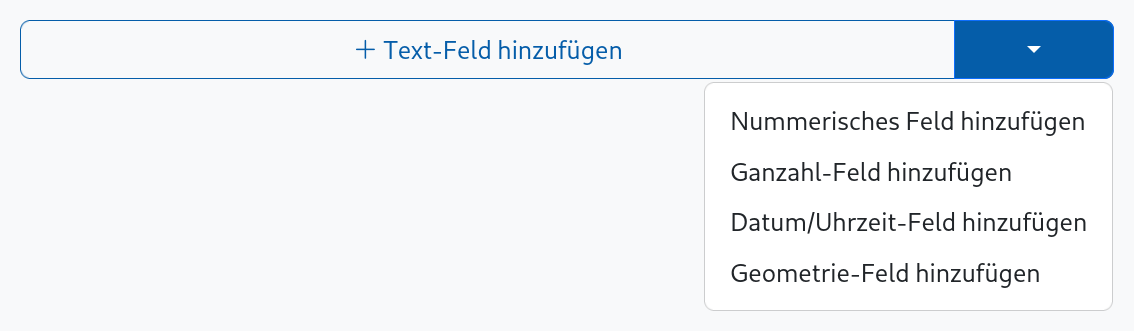
\includegraphics[width=.9\textwidth]{assets/datatype-dropdown.png}
  \caption{Dropdown zum Auswählen des Datentyps von Feldern im Szenario-Modus}
  \label{fig:type-dropdown}
\end{figure}

\plabel{p:ersetzen}
\todo[noline]{ZSMFG: Effizienz / gesparte Klicks}
In der Zielstruktur eingetragene Attribute können nicht ersetzt werden \textbf{(F)}. Dies fiel 4 Teilnehmer:innen auf. Sie versuchten, durch ein erneutes Anklicken eines bestehenden Eintrages den Inhalt mit einer Auswahl aus dem linken Menü zu überschreiben. Aktuell muss zuerst der Button zum Löschen gedrückt werden, wodurch das Feld wieder frei ist und erneut befüllt werden kann. Eine Person versuchte immer wieder eingetragene Attribute zu ersetzen, obwohl sie bereits festgestellt hatte, das dies nicht möglich ist. Zu beachten ist, dass ausschließlich versucht wurde, Attribute zu ersetzen, keine Funktionen. Dies könnte der Art und Weise geschuldet sein, wie eingetragene Attribute dargestellt sind - sie ähneln einem leeren Feld. In Abbildung \ref{fig:buffet-simple} ist der Unterschied zwischen einem leeren Feld, einer ausgewählten Funktion und einem ausgewählten Attribut zu sehen.
\todo{überprüfen ob das noch stimmt falls Bild ausgetauscht}

\plabel{p:drag}
Ebenso oft trat es auf, dass Teilnehmer:innen mittels \textit{Drag \& Drop} \textbf{(G)} Elemente von links nach rechts ziehen wollten. In jedem der 4 Fälle war es die erste Intuition und wurde ausgetestet. Nach der Realisation, dass \textit{Drag \& Drop} noch nicht implementiert ist, konnte der Großteil zur konzipierten Bedienweise übergehen. Dabei sollte zuerst das Zielfeld und dann das gewünschte Attribut, beziehungsweise die gewünschte Funktion, angeklickt werden. Andersrum \todo{wording} ist das ebenso möglich. Eine Person tat sich mit der Transition zu dieser Bedienweise schwer.

\plabel{p:parameterübernahme}
Beim Auswählen von Funktionsüberladungen werden die Parameter von einer Überladung nicht in die nächste übernommen \textbf{(H)}. Vier Personen waren davon verwirrt, dass die ersten, bereits ausgefüllten Parameter, leer sind, sobald eine Überladung mit mehr Parametern ausgewählt wird. Zwei von ihnen merkten an, dass die Anzahl der Parameter auch nach dem Ausfüllen anpassbar sein sollte, wobei eine von ihnen darauf einging dass es schwierig sein könnte, dies konsistent umzusetzen. Ein:e Teilnehmer:in erkannte, dass die zuvor eingetragenen Parameter in der Überladung mit weniger Parametern bestehen bleiben, und entfernte diese manuell, aus Angst dass dies Fehler verursachen könnte.

\begin{figure}[!ht]
  \minipage[t]{.49\textwidth}
  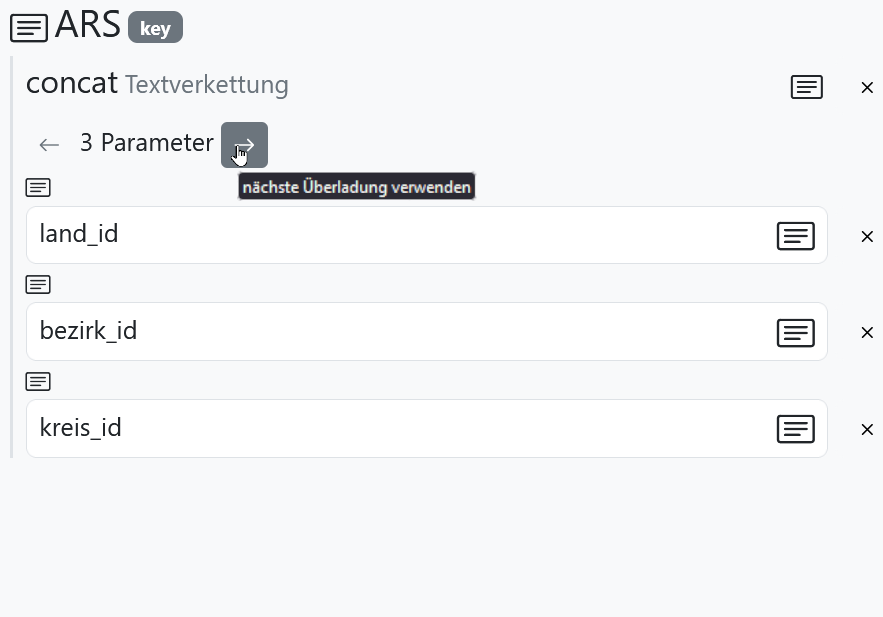
\includegraphics[width=\linewidth]{assets/concat-overload.png}
  \caption{Überladung der Funktion \texttt{concat} (4 Parameter). Der angezeigte Tooltip lautet "nächste Überladung verwenden".}
  \label{fig:concat-overload}
  \endminipage
  \hfill
  \minipage[t]{.49\textwidth}
  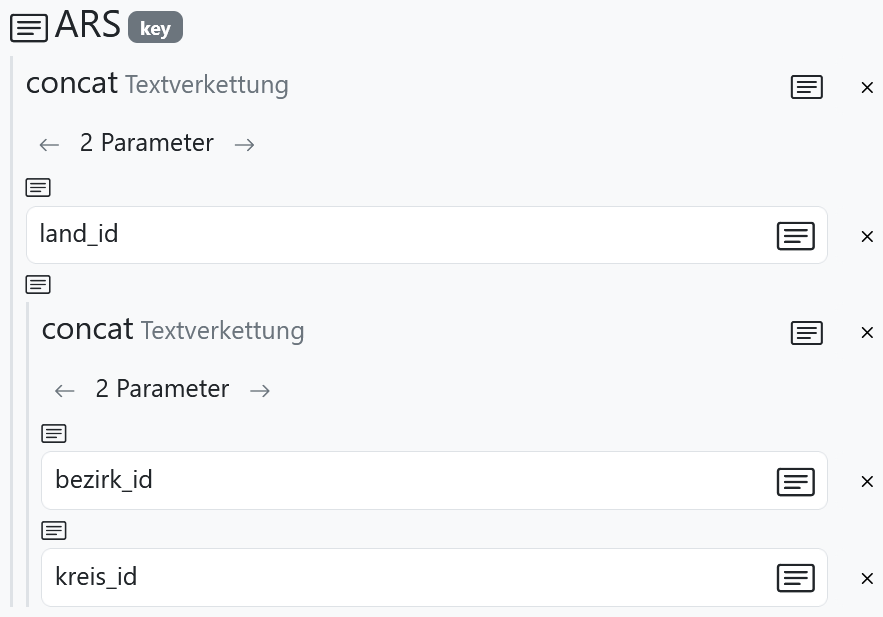
\includegraphics[width=\linewidth]{assets/concat-nested.png}
  \caption{Eine geschachtelte Version der Funktion \texttt{concat}.}
  \label{fig:concat-nested}
  \endminipage
\end{figure}

\plabel{p:overload}
Von den Personen, die keine Probleme mit den Parametern von Überladungen hatten, benutzten 3 die Überladungs-Funktionalität gar nicht. Sie erkannten die Möglichkeit nicht, eine andere Überladung auszuwählen \textbf{(K)}. In Abbildung \ref{fig:concat-overload} und \ref{fig:concat-nested} ist die Funktion \texttt{concat} zu sehen, bei der es zu den genannten Problemen kam. Die 3 Personen, die keine Überladungen benutzten, wählten die in Abbildung \ref{fig:concat-nested} abgebildete Herangehensweise, die zur Folge hat, dass $n-1$ mal die Funktion ausgewählt werden muss, wobei $n$ die Anzahl der Einzelbestandteile ist. Zwei der drei Personen nahmen dies so hin, während die dritte es als "nervig" und "umständlich" bezeichnete. \todo{klingt das bisschen verletzt?} Im Nachhinein wies sie auch darauf hin, dass sie die Pfeile zum Umschalten zwischen Überladungen als ungeeignet errachtet. An dieser Stelle hätte sie eher ein Plus und Minus erwartet, oder vielleicht sogar ein Plus am Ende der Parameterliste platziert. In einer anderen Testsitzung wurde der in Abbildung \ref{fig:concat-overload} zu sehende Tooltip ("nächste Überladung verwenden") kritisiert, da die meisten Menschen nicht wissen, was Überladungen sind. \todo[noline]{ZSMFG: overload zu Anzahl parameter vereinfachen}

\plabel{p:statisch}
Die Angabe von statischen Werten \textbf{(L)} führte in 3 Testsitzungen zu 2 unterschiedlichen Problemen. Statische Werte können anstelle von Attributen oder Funktionen in Eingabefeldern eingegeben werden. Dabei kann der Wert ohne besonderen Syntax eingegeben werden, da es sich im Block-Editor um an den Datentyp angepasste Eingabefelder handelt. Eine Person war sah eine einfache Eingabe nicht als Option an und war sich nicht im Klaren dass dies möglich ist. Zwei weitere Teilnehmer:innen setzten ihre Texteingabe zunächst in Hochkommas, konnten diesen Fehler dann jedoch am Ende relativ schnell beheben. Die beiden zuletzt genannten Personen haben Programmier- und \ac{SQL}-Kenntnisse und nannten diese als Ursprung ihrer Handlung.

\plabel{p:filter}
Der Block-Editor filter automatisch relevante Auswahlmöglichkeiten basierend auf ihrem Datentyp \textbf{(O)}. In 3 Testsitzungen wurde diese Funktionalität missverstanden. Im extremsten Fall konnte die Testperson nichts mit den Datentypen anfangen, und war somit auch nicht in der Lage das Konzept des automatischen Typfilters zu verstehen. In einer anderen Testsitzung wurde zwar realisiert, dass beim Anklicken von Elementen links in der Zielstruktur Felder deaktiviert werden, dieser Effekt wurde allerdings dem falschen Grund zugeschrieben. Die Person war der Meinung, dass der Grund hierfür eine bereits getätigte Auswahl ist. In diesem Fall führte dies dazu, dass die durch die Filterung verursachten Änderungen in der UI äußerst untransparent wirkten. Auffällig war, dass alle 3 Teilnehmer:innen von links nach rechts arbeiteten, das heißt, es fiel ihnen schwerer den vollen Effekt der Filterfunktion zu verstehen. Eine dieser Personen äußerte sogar den Wunsch, die Liste der Funktionen zu filtern, erkannte aber nicht, wie dies funktioniert. Wenn die Oberfläche von rechts nach links benutzt wurde, trat dieses Problem nicht auf, es gab aber auch Teilnehmer:innen, die von von links nach rechts arbeiteten, und denen die Funktionsweise klar wurde. Eine:r von ihnen ging daraufhin sogar dazu über, zuerst das Feld rechts auszuwählen, und dann das einzufügende Element links rauszusuchen.

\subsubsection{Darstellungsprobleme}

Auch die Darstellung von Informationen innerhalb des Block-Editors führte zu Problemen. Es wurden 8 Darstellungsprobleme identifiziert, welche von unklaren Bezeichnungen bis hin zu Icons reichen.

\plabel{p:icons}
Abbildung \ref{fig:icons} zeigt die vom Block-Editor verwendeten Icons für Datentypen \textbf{(B)}. Diese werden wie in Abbildung \ref{fig:attribute-source} und \ref{fig:attribute-target} verwendet, um über den Datentyp von Attributen, Funktionen und Feldern zu informieren. Im Rahmen von 5 Testsitzungen wurden die Icons missverstanden oder führten zu Verwirrungen. Da sich die Icons für Ganz- und Gleitkommazahlen nicht voneinander unterscheiden, kam es zu Verwechslungen. Eine Person wählte beispielsweise im dritten Szenario ein Gleitkommazahl-Feld aus (im Dropdown als "numerisch" bezeichnet, siehe Abbildung \ref{fig:type-dropdown}), um eine Hausnummer einzusetzen, obwohl es sich bei der Hausnummer um eine Ganzzahl handelt.  Drei Teilnehmer:innen sahen das Icon für Booleans als zwei interaktive Schalter an, und versuchten, sie zu bedienen. Eine Person empfand das Icon für den Datentyp Text als Button, über den mehr Informationen über ein Attribut oder eine Funktion abegrufen werden könnten. Eine weitere Person empfand die Icons als guten Ort, um einen Ausschnitt aus der Quelltabelle abzurufen.

\begin{figure}
  \centering
  \begin{tikzpicture}
    \tikzset{icon/.style={outer xsep=4.5em, outer ysep=1em, minimum height=3em}}
    \tikzset{label/.style={font=\footnotesize}}
    \node [icon] (text)  at (0, 0)       {\includesvg[width=2em]{assets/bi-card-text.svg}};
    \node [icon] (int)   at (text.east)  {\includesvg[width=2em]{assets/bi-123.svg}};
    \node [icon] (float) at (int.east)   {\includesvg[width=2em]{assets/bi-123.svg}};
    \node [icon] (bool)  at (float.east) {\includesvg[width=2em]{assets/bi-toggles.svg}};
    \node [icon] (dt)    at (bool.east)  {\includesvg[width=2em]{assets/bi-calendar-week.svg}};
    \node [icon] (geom)  at (dt.east)    {\includesvg[width=2em]{assets/bi-pin-map.svg}};
    \node [label] at (text.south)  {Text};
    \node [label] at (int.south)   {Ganzzahl};
    \node [label] at (float.south) {Gleitkommazahl};
    \node [label] at (bool.south)  {Boolean};
    \node [label] at (dt.south)    {Datum/Zeit};
    \node [label] at (geom.south)  {Geometrie};
  \end{tikzpicture}
  \caption{Die im Block-Editor verwendeten Icons für Datentypen \parencitealias{bootstrapIcons}.}
  \label{fig:icons}
\end{figure}

\plabel{p:attribute}
Die Anzeige von Attributen in der Zielstruktur weicht von der im Auswahlmenü ab \textbf{(D)}. Im Auswahlmenü wird sowohl der Name, als auch der Schlüssel von Attributen angezeigt, während im mittleren Bereich nur noch der Schlüssel angezeigt wird. Dies fiel 5 Teilnehmer:innen auf, zumeist im dritten Szenario, wahrscheinlich weil sich dort die Inhalte mehr unterscheiden. Abbildung \ref{fig:attribute-source} und \ref{fig:attribute-target} stellen dies beispielhaft dar. "strassenname" ist der Name des Attributs der Objektklasse, während "description" der Schlüssel ist. Sobald das Attribut im Ziel erscheint, wird nur noch der Schlüssel angezeigt. Besonders im Fall der Standardfelder \footnote{\texttt{key, ndx, typ, dsc, cmt, beg, fin}, Vgl. \ref{sec:theory-s4d-reality}}, kann dieser stark vom Name abweichen. Fünf Personen waren davon verwirrt.

\begin{figure}[!ht]
  \minipage[t]{.38\textwidth}
  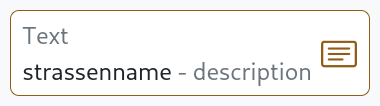
\includegraphics[width=\linewidth]{assets/attribute-source.png}
  \caption{Ein Attribut im Auswahlmenü.}
  \label{fig:attribute-source}
  \endminipage
  \hfill
  \minipage[t]{.60\textwidth}
  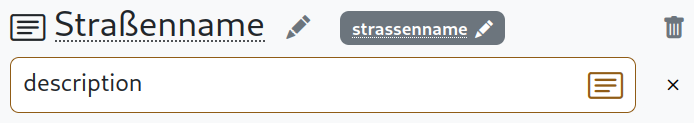
\includegraphics[width=\linewidth]{assets/attribute-target.png}
  \caption{Ein Attribut in der Zielstruktur - es wird nur der Schlüssel dargestellt.}
  \label{fig:attribute-target}
  \endminipage
\end{figure}

\plabel{p:speichern}
\plabel{p:mitte}
\plabel{p:meta}
\plabel{p:queryables}
\plabel{p:functionlist}

\subsubsection{Inhaltliche Probleme}

\plabel{p:parameter}
\plabel{p:quelle}
\plabel{p:functions}
\plabel{p:präfix}

\subsubsection{Technische Probleme}

\plabel{p:scroll}
